\chapter{Robot Firmware Implementation}
\label{Chapter 5}
\lhead{Chapter 5. \emph{Robot Firmware Implementation}}

With the creation of the software embedded Bluetooth stack and the \textit{ExplorerBot} test robot platform hardware, it was neccesary to integrate these two components into a functional prototype. By using the Bluetooth stack in a real-world, practical application while it was being developed, the quality, effectiveness and completeness of the stack could be evaluated.

\section{Build Dependencies}

To match the Bluetooth stack, each module was written in the C language, and targeted at the free open source AVR-GCC compiler and avr-libc library. A standard \textit{makefile} included with the firmware allows for command line control over the building of the project files into a set of binaries which can then be programmed into the target microcontroller for use via the command \texttt{make all}. The following tools are required to build the firmware under Windows:

\begin{itemize}
	\item The \textbf{WinAVR 20100101} release download, or Windows binaries of the \textbf{GNU Shell Utilities}
	\item The latest \textbf{AVR Toolchain} release from Atmel (Included with Atmel's free \textit{AVRStudio 5} software)
\end{itemize}

Under Debian Linux environments, the following packages are required:

\begin{itemize}
	\item \textbf{gcc-avr} 
	\item \textbf{binutils-avr}
	\item \textbf{avr-libc}
	\item \textbf{avrdude}
\end{itemize}

Which can be installed via the command prompt using the command \texttt{sudo apt-get install gcc-avr binutils-avr avr-libc avrdude}.

\section{Firmware Overview}

The completed firmware of the \textit{ExplorerBot} prototype was developed in a modular manner, to match the corresponding hardware components. This top-down methodology ensured that each portion of the firmware could be mocked up, tested and integrated as needed. Additionally, seperating out the firmware components into logical modules gave the final firmware a level of flexibility which should allow for easy modification to suit any hardware changes made to those of the prototype. The completed set of modules (see Figure \ref{fig:robotblockfw}) served as the complete firmware for the robot.

\begin{figure}[H]
	\vspace{1em}
	\centering
		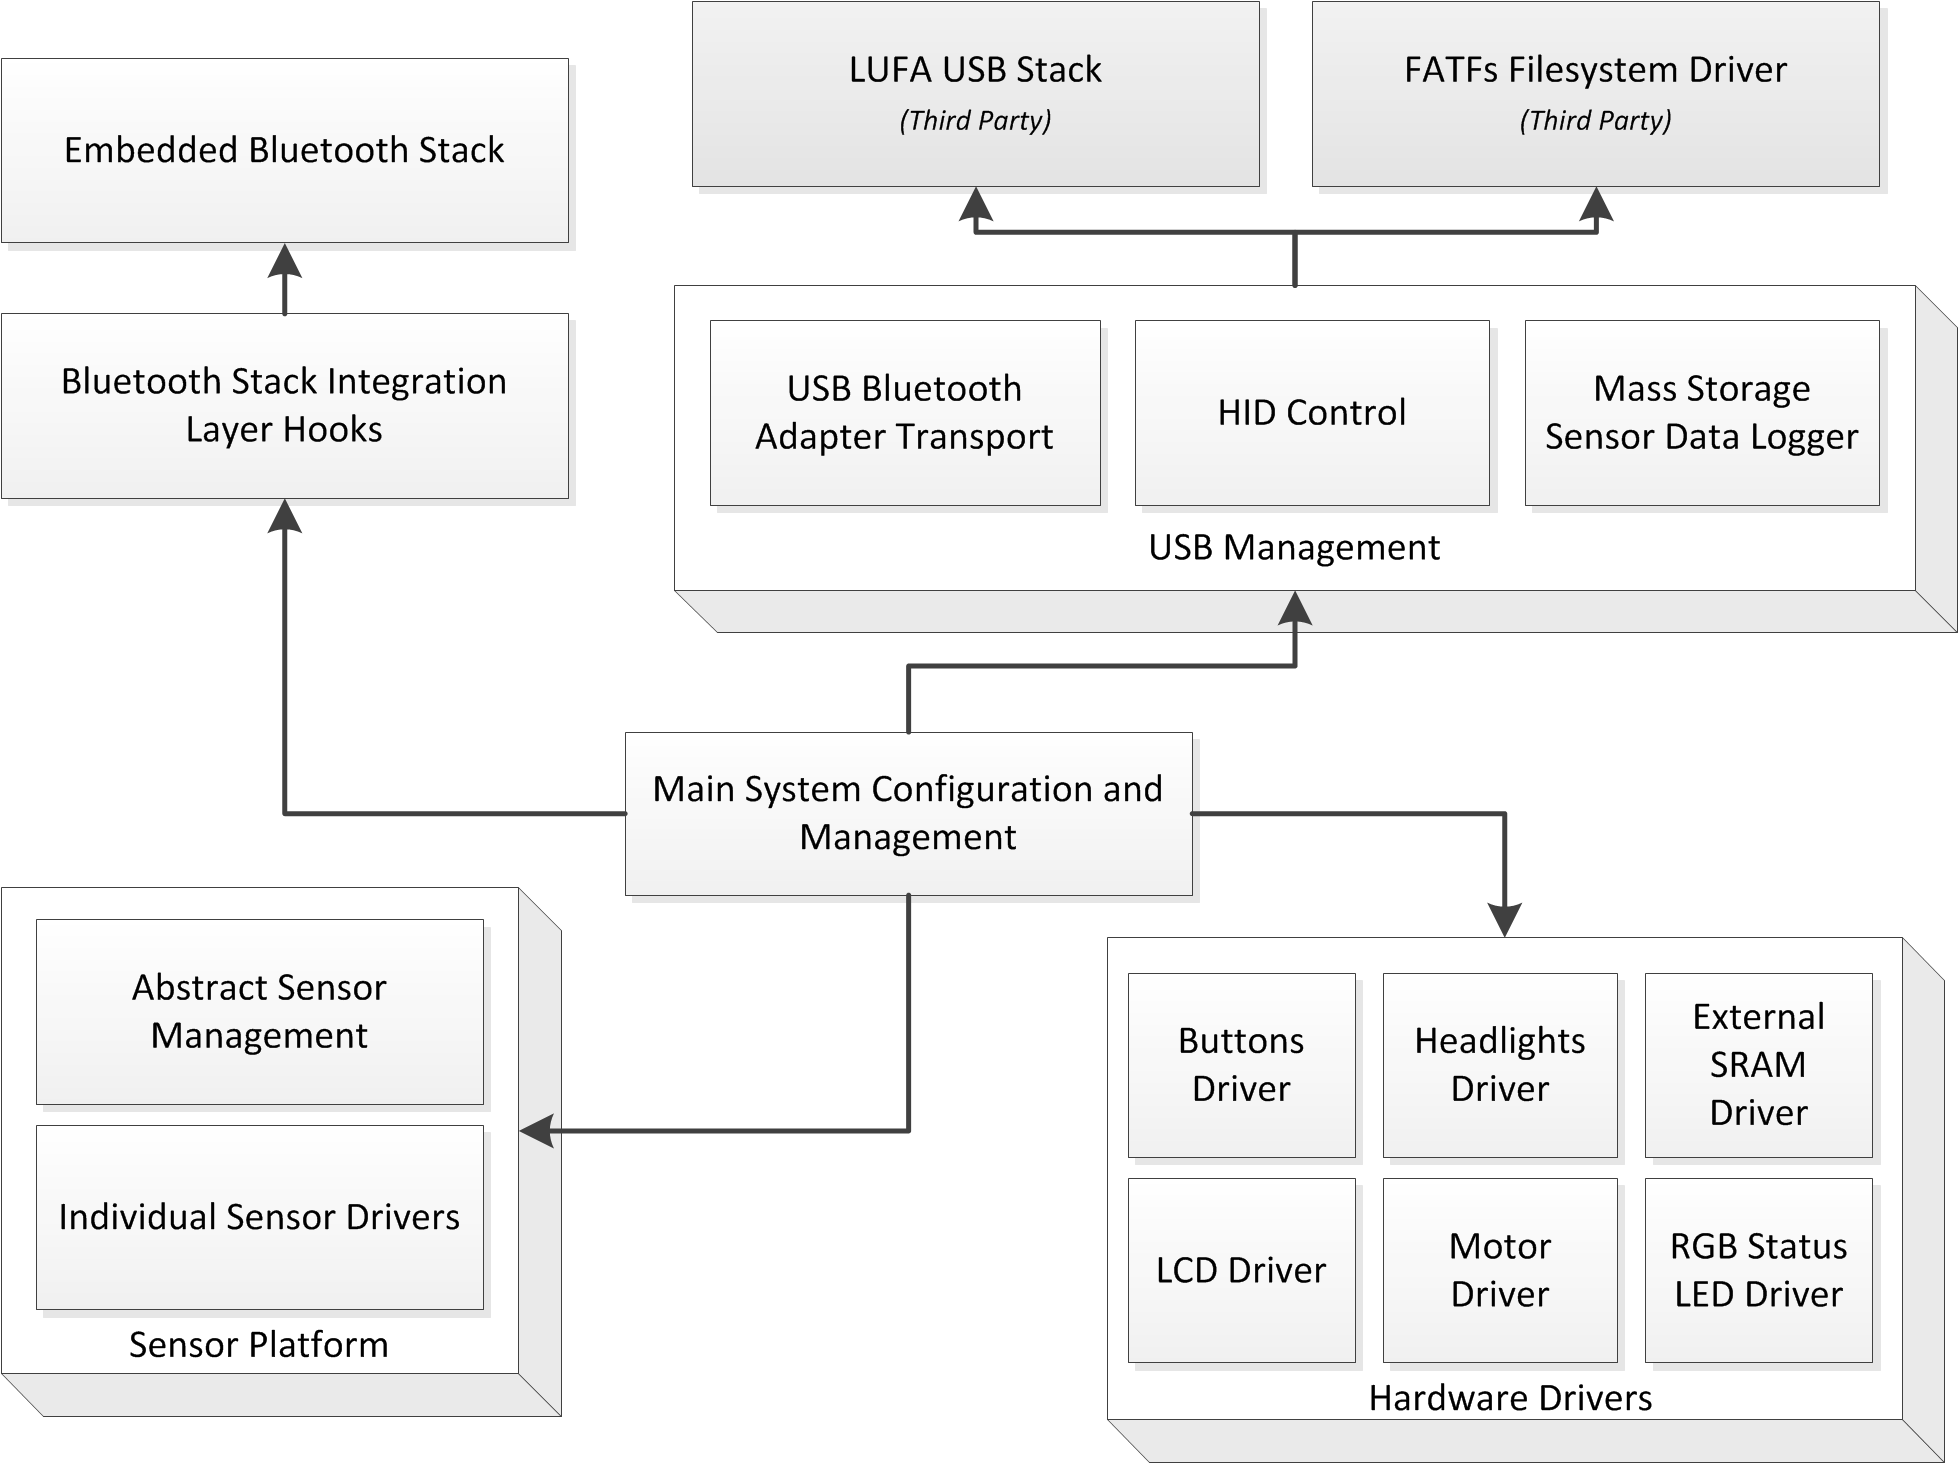
\includegraphics[width=140mm]{./Figures/FirmwareBlockDiagram.png}
	\rule{35em}{0.5pt}
	\caption[Firmware Block Diagram]{Robot Firmware Block Diagram}
	\label{fig:robotblockfw}
\end{figure}

\section{Firmware Modules}

In this section, each of the robot firmware's main software modules are listed and described in additional detail so that the overall design and implementation of the firmware can be further understood.

\FloatBarrier
\subsection{Main System Control and Configuration}

% TODO

\FloatBarrier
\subsection{Hardware Drivers}

% TODO

\FloatBarrier
\subsection{Sensor Platform}

% TODO

\FloatBarrier
\subsubsection{Abstract Sensor Management}

% TODO

\FloatBarrier
\subsubsection{Individual Sensor Drivers}

% TODO

\FloatBarrier
\subsection{USB Management}

% TODO

\FloatBarrier
\subsubsection{Bluetooth Adapters}

% TODO

\FloatBarrier
\subsubsection{HID Devices}

% TODO

\FloatBarrier
\subsubsection{Mass Storage Devices}

% TODO

\FloatBarrier
\subsection{Bluetooth Management}

% TODO

\FloatBarrier
\subsubsection{Stack Integration Layer}

% TODO

\FloatBarrier
\subsubsection{Bluetooth Stack}

% TODO

\FloatBarrier
\subsection{Third Party Modules}

% TODO

\FloatBarrier
\subsubsection{LUFA}

% TODO

\FloatBarrier
\subsubsection{FatFS}

% TODO
